\section{Results}

\begin{figure}[tp]
\centering
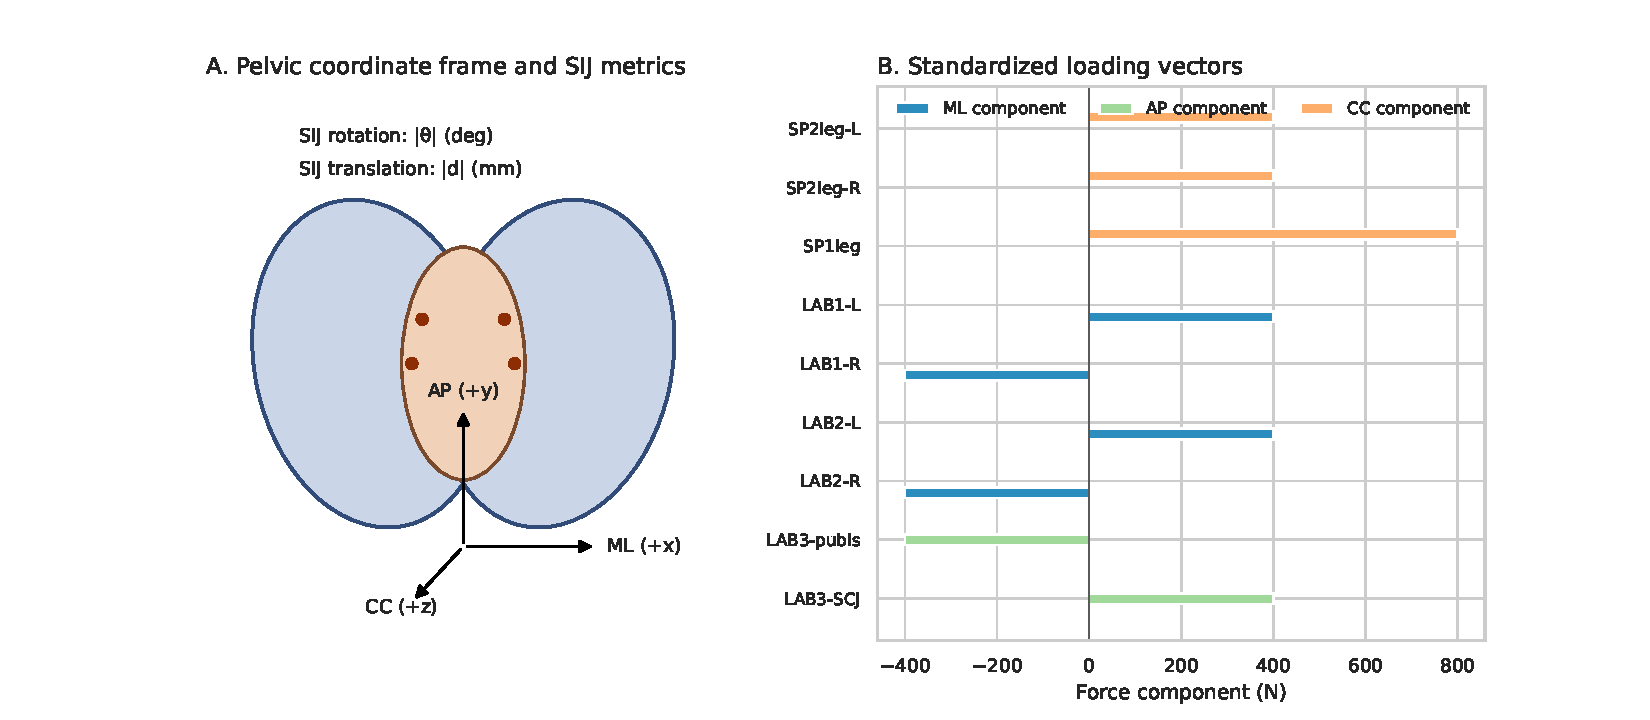
\includegraphics[width=\textwidth,height=0.38\textheight,keepaspectratio]{figures/Fig1_anatomy_coordinates_loads.pdf}
\caption{\textbf{Pelvic anatomical assembly, SIJ coordinate triad with 6 degrees of freedom, and standardized 3D loading configurations.} 
(A) 3D finite-element pelvic assembly showing the bilateral sacroiliac joint (SIJ) articular cartilages (orange), the superior S1 sacral facet constrained via a Dirichlet boundary penalty condition ($\mathbf{u} = \mathbf{0}, \gamma = 10^6\;\text{N/mm}$; green plate), and the anterior fibrocartilaginous pubic symphysis disc (purple). Overlays delineate the primary morphometric triad: anteroposterior inlet diameter (conjugata vera $d_{\text{AP}}$, dashed blue line), biischiadic interspinous width ($w_{\text{biisch}}$, dashed orange line), and subpubic arch angle ($\alpha_{\text{subpubic}}$, magenta). 
(B$_1$) Exploded 3D view of the left SIJ articulation (ilium laterally offset by $+40\;\text{mm}$) exposing the sacral auricular cartilage (orange), iliac articulation facet, contact centroid ($\mathbf{p}_c$), and the orthogonal anatomical coordinate triad: mediolateral ($\hat{\mathbf{x}}_{\text{ML}}$, green), anteroposterior ($\hat{\mathbf{y}}_{\text{AP}}$, blue), and craniocaudal ($\hat{\mathbf{z}}_{\text{CC}}$, vermilion). 
(B$_2$) Definition of the 6 SIJ degrees of freedom (6 DOFs). Three rotational DOFs follow an intrinsic Cardan $XYZ$ sequence: nutation ($\theta_{\text{nut}} = \alpha_x$, transverse ML axis; $+ > 0$ denotes anterior sacral promontory tilt relative to ilium / self-bracing), abduction/out-flare ($\theta_{\text{abd}} = \beta_y$, AP axis; lateral iliac wing opening), and axial rotation/torsion ($\theta_{\text{rot}} = \gamma_z$, CC axis; internal axial twist). Three translational DOFs track motion at contact point $\mathbf{p}_c$: mediolateral distraction/compression ($d_{\text{ML}} = dx$), anteroposterior gliding/shear ($d_{\text{AP}} = dy$), and vertical craniocaudal shear ($d_{\text{CC}} = dz$). Scalar resultant rotations $|\boldsymbol{\theta}|$, resultant translations $|\mathbf{d}|$, and bilateral translation asymmetry $\Delta_{\text{asym}}$ are defined in the bottom legend. 
(C$_1$--C$_2$) Habitual locomotor regimes: symmetrical two-leg stance (SP2leg; $+400\;\text{N}$ per acetabular notch, resultant $+800\;\text{N}$ reacting against the constrained sacral base, promoting physiological self-bracing nutation $\theta_{\text{nut}} \approx 1.06^\circ$) and single-leg stance (SP1leg; $+800\;\text{N}$ unilateral vertical ground reaction on the right acetabulum with unsupported contralateral hemi-pelvis, inducing a marked bilateral asymmetry jump $\Delta_{\text{asym}} \approx 2.01\;\text{mm}$). 
(D$_1$--D$_3$) Parturition-motivated proxy loads (birth canal transit stages): labor phase 1 (LAB1; inlet compression proxy, opposing $\pm 400\;\text{N}$ mediolateral pair on inner pectineal ring); labor phase 2 (LAB2; ischial tuberosity distraction proxy, $\pm 400\;\text{N}$ outward mediolateral pair yielding maximum outward transverse expansion $\Delta\text{ML} = +0.15\;\text{mm}$); and labor phase 3 (LAB3; outlet AP distraction proxy, $\pm 400\;\text{N}$ opposing anteroposterior forces acting between anterior pubis and posterior sacrococcygeal complex, eliciting high sagittal rotation $|\boldsymbol{\theta}| = 1.34^\circ$). Mathematical formulations for the continuum boundary value problem, landmark extractions, rigid kinematic registration, and Cardan angle extractions are detailed in Appendix~\ref{app:mathematical_formulation}.}
\label{fig:overview}
\end{figure}

\subsection{Cohort completeness and morphometric sexual dimorphism}
The analyzed cohort comprised 278 human pelvic models (150 female, 128 male; age 53.9 $\pm$ 19.3 years, range 16--91). All 278 datasets exhibited complete records across demographic metadata, eight 3D anatomical dimensions, and finite-element kinematic outcomes (Table~\ref{tab:cohort}). Morphometric comparisons confirmed characteristic pelvic sexual dimorphism: female pelves exhibited significantly larger mean anteroposterior inlet diameter ($121.04 \pm 10.02$ vs.\ $112.34 \pm 9.07$~mm), biischiadic outlet width ($109.87 \pm 7.13$ vs.\ $97.71 \pm 7.06$~mm), and subpubic arch angle ($85.80 \pm 6.14^\circ$ vs.\ $69.11 \pm 5.26^\circ$), despite having lower total pelvic bone volume ($736.79 \pm 105.99$ vs.\ $925.28 \pm 126.99\;\text{cm}^3$) and lower global scale factors ($0.92 \pm 0.05$ vs.\ $1.00 \pm 0.05$) than male pelves.

\subsection{Functional load-dependence: locomotor self-bracing versus asymmetric shear (H1)}
Sacroiliac joint kinematics varied markedly across loading regimes (Table~\ref{tab:microsummary}; Fig.~\ref{fig:loadprofiles}). Bipedal standing (SP2leg) engaged physiological nutation (median $\theta_{\text{nut}} = 1.062^\circ$ [IQR 0.653, 1.522]), maintaining low bilateral translation asymmetry ($0.215$~mm [0.093, 0.347]) and moderate resultant motion ($|\boldsymbol{\theta}| = 1.692^\circ$ [1.211, 2.451]; $|\mathbf{d}| = 1.299$~mm [0.971, 1.625]).

Transition to single-leg stance (SP1leg) produced the highest kinematic demand among the evaluated states, driving resultant rotation to $2.516^\circ$ [1.981, 3.137] and translation to $1.755$~mm [1.458, 2.053]. Unilateral acetabular support induced a marked increase in bilateral translation asymmetry, rising from $0.215$~mm in SP2leg to $2.013$~mm [1.423, 2.548] in SP1leg (Fig.~\ref{fig:loadprofiles}D). While sagittal nutation remained elevated ($1.160^\circ$ [0.819, 1.619]), unilateral vertical support imposed substantial frontal pelvic tilt (abduction $\theta_y = 1.582^\circ$ [1.195, 1.977]), generating differential shear across the pelvic arch.

\begin{table}[H]
\centering
\caption{SIJ micromotion summary by load case across 278 subjects. Values represent median [interquartile range].}
\label{tab:microsummary}
\StdTableInput{tables/generated/table3_micromotion_summary.tex}
\end{table}

\begin{figure}[H]
\centering
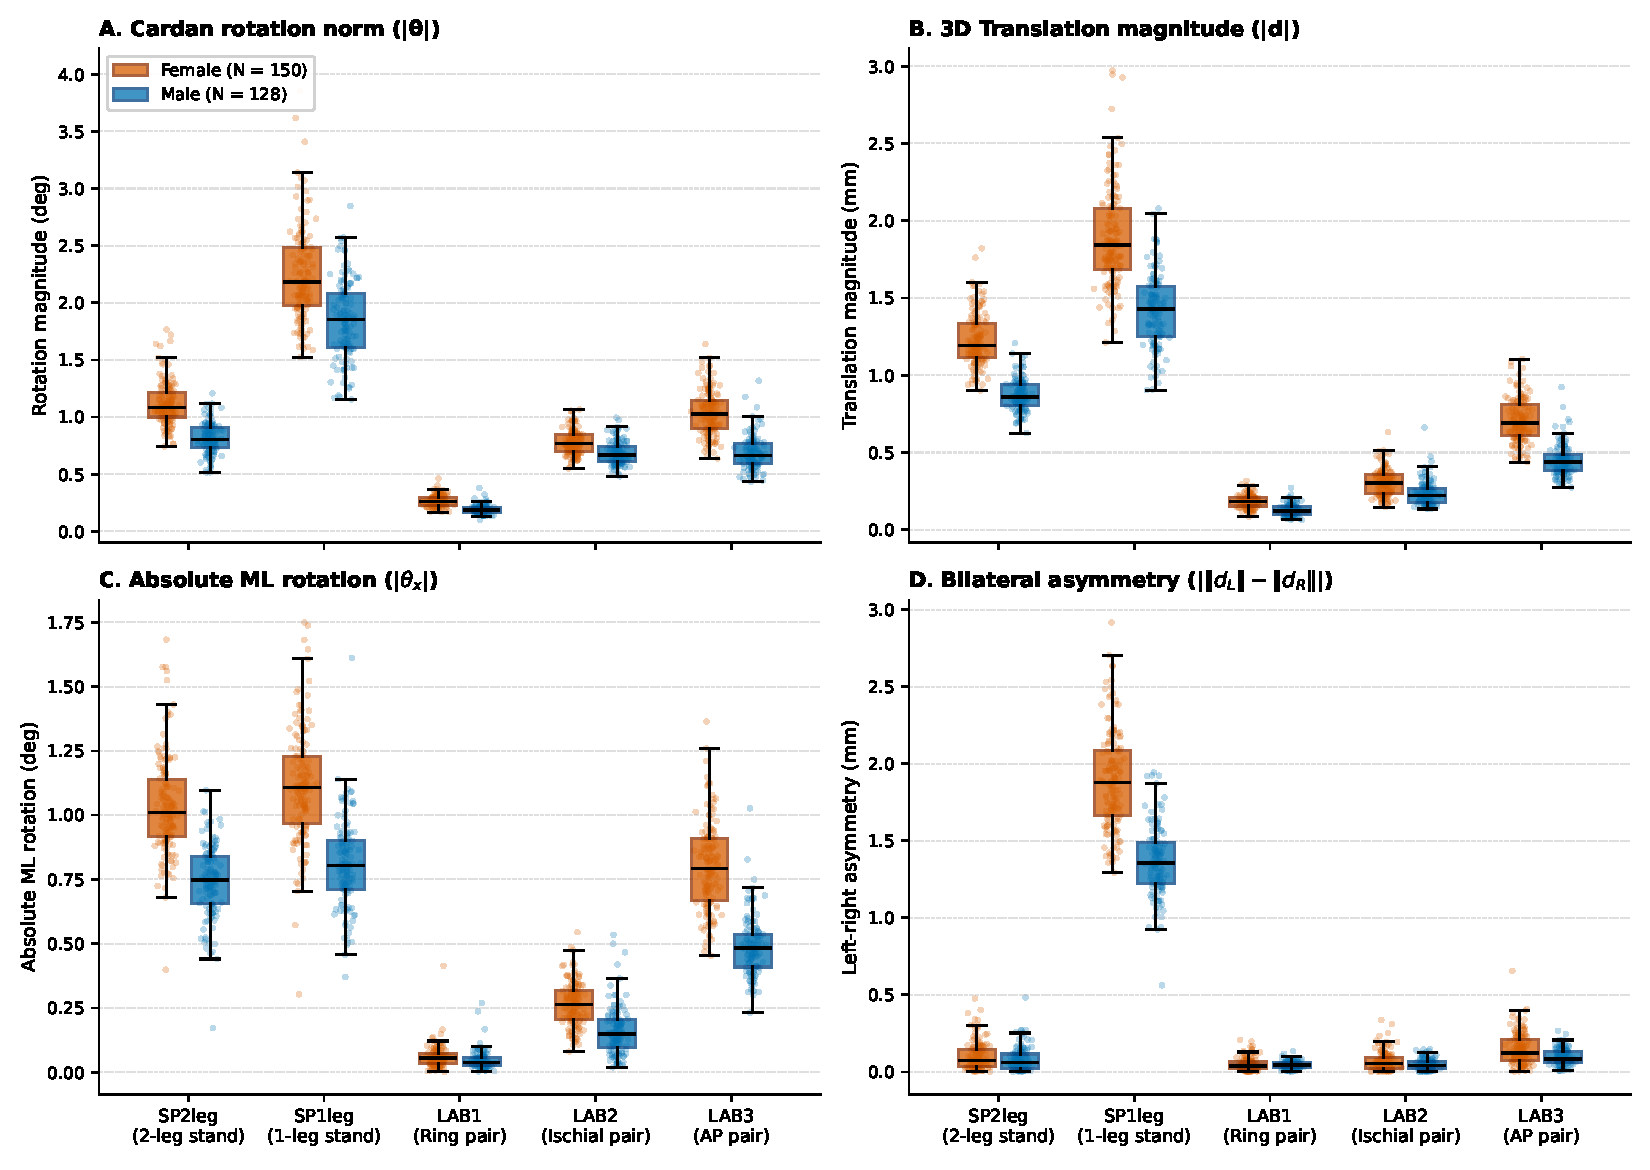
\includegraphics[width=0.98\textwidth]{figures/Fig2_primary_load_profiles.pdf}
\caption{\textbf{Primary SIJ kinematic distributions across locomotor and parturition load regimes.} Raincloud distribution dashboard showing: (A) 3D resultant rotation magnitude ($|\boldsymbol{\theta}|$, deg), (B) 3D resultant translation magnitude ($|\mathbf{d}|$, mm), (C) sagittal nutation angle ($\theta_{\text{nut}}$, deg), and (D) bilateral translation asymmetry ($|d_{\text{left}} - d_{\text{right}}|$, mm). Boxplots depict medians and interquartile ranges; dashed reference lines indicate quiet stance baselines (SP2leg). Note the reduction in nutation under simulated labor (C) and the marked elevation in bilateral asymmetry during single-leg stance (D).}
\label{fig:loadprofiles}
\end{figure}

\subsection{Directional kinematic contrasts in 3D state space (H2)}
Under parturition-motivated configurations (LAB1--LAB3), SIJ kinematics exhibited directional re-routing rather than uniform scaling (Table~\ref{tab:microsummary}; Fig.~\ref{fig:directional}). In contrast to stance, sagittal nutation decreased under internal ring expansion, dropping to $0.432^\circ$ [0.257, 0.731] in LAB1 and $0.412^\circ$ [0.247, 0.630] in LAB2 (Fig.~\ref{fig:loadprofiles}C).

Decomposition of within-subject displacement differences relative to SP2leg demonstrated directional anisotropy (Fig.~\ref{fig:directional}A; Supplementary Table S1). Single-leg stance selectively increased vertical shear ($\Delta\text{CC} = +0.394$~mm, 95\% CI 0.347 to 0.434, $p < 10^{-40}$) and anteroposterior translation ($\Delta\text{AP} = +0.072$~mm, 95\% CI 0.045 to 0.096, $p < 10^{-20}$), while mediolateral displacement showed no significant shift ($\Delta\text{ML} = +0.005$~mm, $p = 0.095$). Conversely, internal ring compression (LAB1) produced an abrupt reduction in craniocaudal shear ($\Delta\text{CC} = -0.850$~mm, 95\% CI $-0.881$ to $-0.811$) while channeling displacement into transverse outward distraction ($\Delta\text{ML} = +0.086$~mm, 95\% CI 0.077 to 0.095, $p < 10^{-30}$). Circumferential dilation (LAB2) similarly suppressed vertical shear ($\Delta\text{CC} = -0.903$~mm, 95\% CI $-0.931$ to $-0.853$) while augmenting both transverse distraction ($\Delta\text{ML} = +0.145$~mm, 95\% CI 0.132 to 0.160) and sagittal gliding ($\Delta\text{AP} = +0.163$~mm, 95\% CI 0.102 to 0.213).

Projecting these responses into a 2D kinematic state space ($\Delta\text{ML}$ vs.\ $\Delta\text{CC}$; Fig.~\ref{fig:directional}B) highlights the directional contrast: locomotor stance contrasts populate the vertical shear axis, whereas parturition proxies diverge along the transverse distraction axis.

\begin{figure}[H]
\centering
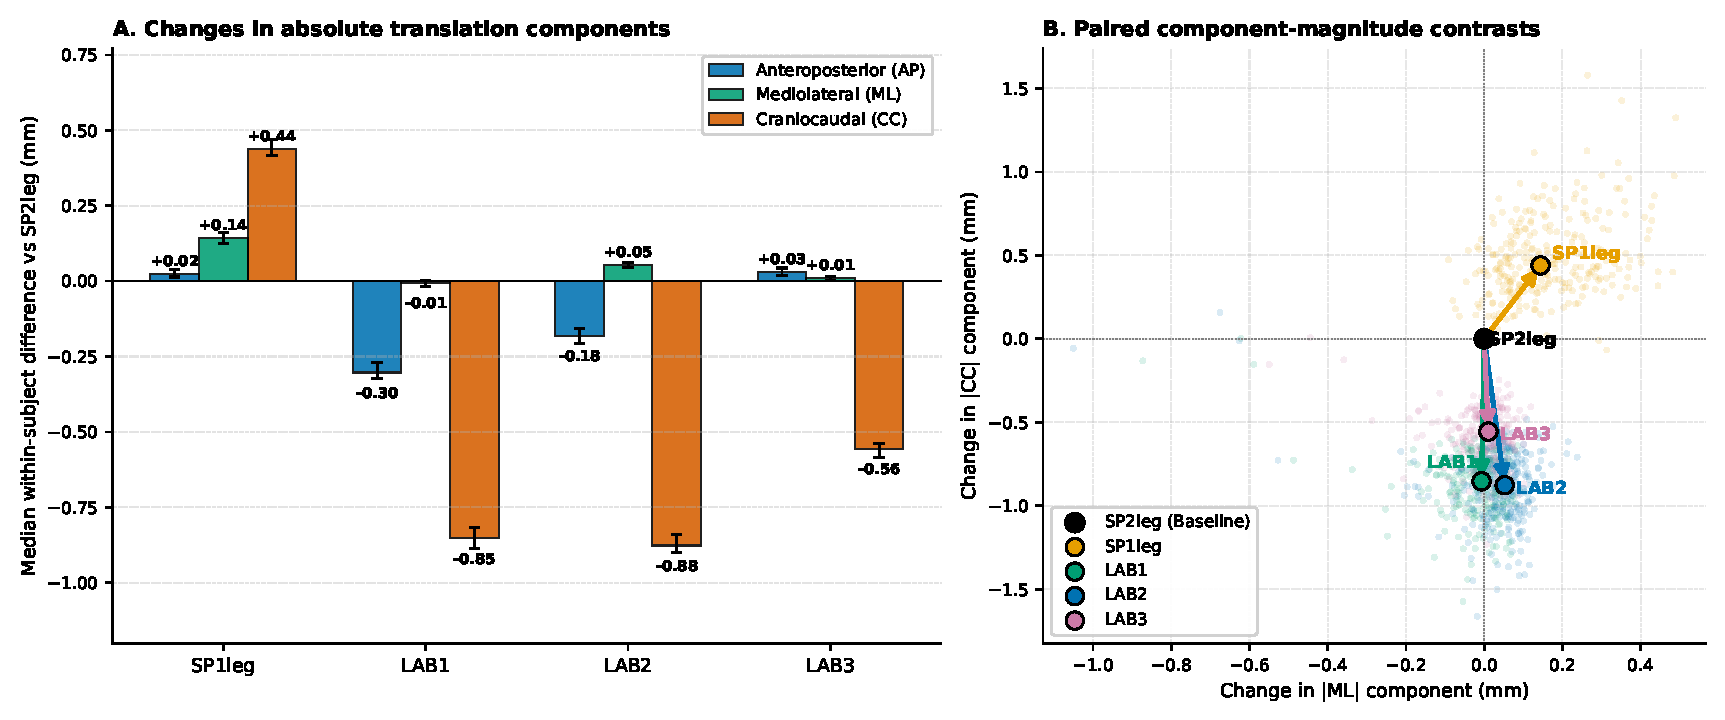
\includegraphics[width=0.95\textwidth]{figures/Fig3_directional_rerouting.pdf}
\caption{\textbf{Directional translation differences and 2D state-space contrast.} (A) Within-subject translation shifts ($\Delta = \text{Load} - \text{SP2leg}$) for anteroposterior (AP, blue), mediolateral (ML, green), and craniocaudal (CC, vermilion) axes. Error bars indicate bootstrap 95\% confidence intervals; asterisks denote significant median shifts after BH-FDR correction ($q < 0.05$). (B) Kinematic state-space contrast mapping transverse shifts ($\Delta\text{ML}$) against vertical shear shifts ($\Delta\text{CC}$), highlighting the functional divergence between locomotor vertical shear and obstetric transverse ring compliance.}
\label{fig:directional}
\end{figure}

\subsection{Sex-related differences and morphometric associations (H3)}
In unadjusted models conditioned only on age (Model 0; Eq.~\ref{eq:m0}), female pelves demonstrated greater translation magnitude under all parturition configurations: $+0.364$~mm in LAB1 (SE $= 0.030, p < 10^{-30}$), $+0.414$~mm in LAB2 (SE $= 0.033, p < 10^{-35}$), and $+0.344$~mm in LAB3 (SE $= 0.031, p < 10^{-25}$). Adjusting for total pelvic bone volume (Model 1; Eq.~\ref{eq:m1}) attenuated the female surplus to $+0.295$~mm in LAB1, $+0.329$~mm in LAB2, and $+0.279$~mm in LAB3 ($p < 10^{-9}$ for all). 

Further adjustment for the morphometric triad (Model 2; Eq.~\ref{eq:m2}: AP diameter, biischiadic width, and subpubic arch angle) reduced the conditional difference (female minus male) to $+0.224$~mm in LAB1 ($\text{SE} = 0.078$, 95\% CI 0.070 to 0.378, $p = 0.0042$), $+0.193$~mm in LAB2 ($\text{SE} = 0.083$, 95\% CI 0.031 to 0.355, $p = 0.0196$), and $+0.231$~mm in LAB3 ($\text{SE} = 0.080$, 95\% CI 0.075 to 0.388, $p = 0.0038$; Fig.~\ref{fig:sexeffects}A,B; Supplementary Table S3). Across Model 2, multicollinearity diagnostics confirmed acceptable variance inflation factors: female sex ($\text{VIF} = 5.55$), subpubic angle ($\text{VIF} = 4.76$), biischiadic width ($\text{VIF} = 3.03$), pelvic volume ($\text{VIF} = 2.62$), AP diameter ($\text{VIF} = 1.59$), and age ($\text{VIF} = 1.55$), all well below the standard threshold of 10. Rotational dimorphism was strongest in outlet distraction (LAB3: $+0.627^\circ$, 95\% CI 0.206 to 1.048, BH-FDR $p = 0.007$).

In pooled cluster-robust models across all load regimes, female sex retained significant positive associations for both rotation ($+0.450^\circ$, $p = 0.020$) and translation ($+0.254$~mm, $p < 0.001$; Table~\ref{tab:allometry}A). Morphometric associations revealed that enhanced compliance is linked with anterior arch architecture: LAB1 translation correlated positively with the subpubic arch angle (Spearman $r = 0.52, p = 2.2 \times 10^{-20}$; Fig.~\ref{fig:sexeffects}C), indicating that wider anterior arch geometry facilitates outward compliance of the dorsal sacroiliac joints.

\begin{figure}[H]
\centering
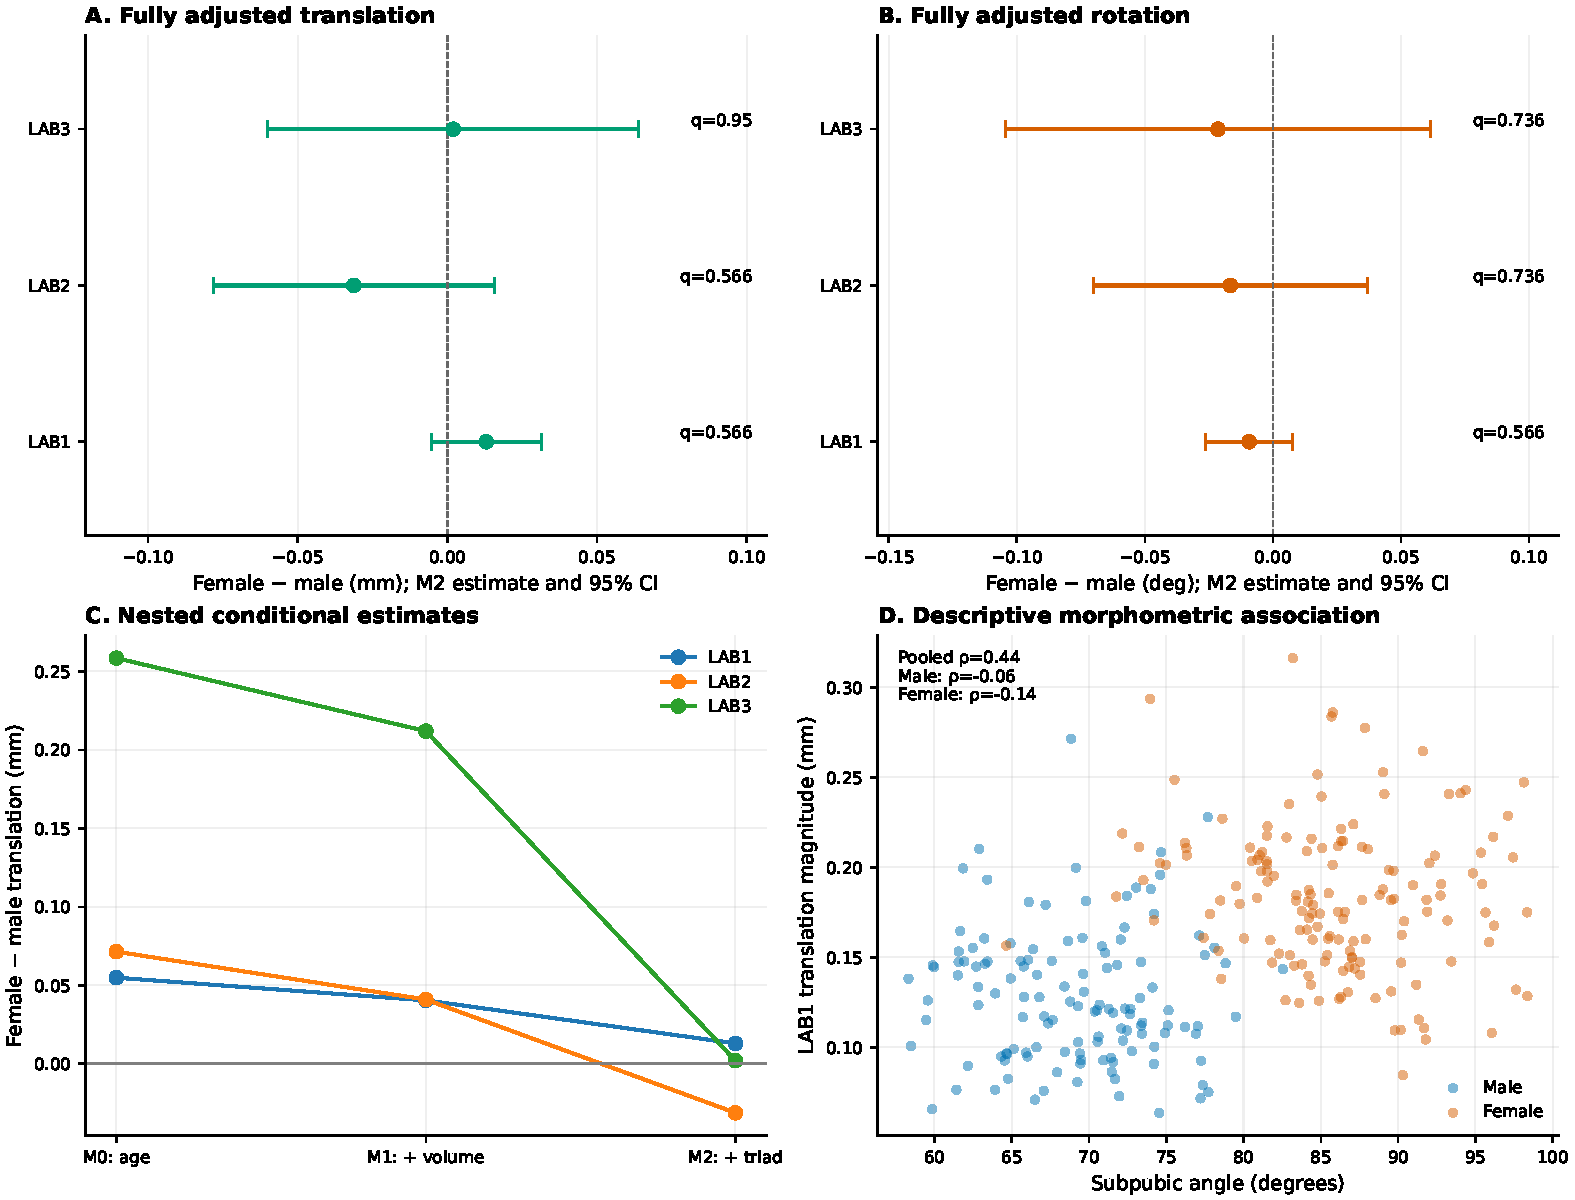
\includegraphics[width=0.98\textwidth]{figures/Fig4_sex_effects_lab.pdf}
\caption{\textbf{Sex-related differences under parturition loading and morphometric associations.} (A) Forest plot of adjusted female-minus-male differences (95\% CI) for translation magnitude (green circles) and rotation magnitude (orange squares) across LAB1--LAB3 from multivariable robust OLS models. (B) Kernel density distributions of covariate-adjusted translation in LAB1 for females (vermilion) and males (blue). (C) Morphometric association scatterplot of LAB1 translation magnitude versus subpubic arch angle across the cohort ($r = 0.52, p = 2.2 \times 10^{-20}$).}
\label{fig:sexeffects}
\end{figure}

\subsection{Variance channels: structural geometry versus material heterogeneity (H4)}
Decomposition of between-subject variance across the three matched simulation variants revealed that macroscopic skeletal geometry accounts for the predominant share of population dispersion (Fig.~\ref{fig:variance}; Supplementary Table S2). The shape-only model reproduced $98.7\%$ to $102.1\%$ (overall median $100.46\%$) of full-model variance across all load cases and kinematic degrees of freedom. Values slightly exceeding 100\% reflect sample-variance ratios derived from separate simulation datasets, signifying near-complete variance retention by skeletal geometry.

Paired subject-level diagnostics between the Full and Shape-Only models confirmed close individual correspondence across all load regimes. For resultant translation magnitude, the coefficient of determination against the 1:1 identity line was $R^2 \ge 0.994$, with Pearson correlation $r \ge 0.997$, Spearman rank correlation $r_s \ge 0.996$, $\text{RMSE} \le 0.031$~mm, and $\text{MAE} \le 0.021$~mm. For resultant rotation, concordance was similarly high ($R^2 \ge 0.999$, $r \ge 0.999$, $\text{RMSE} \le 0.023^\circ$, $\text{MAE} \le 0.015^\circ$).

In contrast, the material-only model (isolating CT-derived bone mineral density and elastic modulus heterogeneity on the unmapped reference geometry) accounted for a small fraction of population variance, ranging from $0.001\%$ to $0.317\%$ (overall median $0.033\%$). For resultant rotation and translation, material-only variance fractions remained below $0.053\%$ and $0.295\%$, respectively. Under parturition-motivated configurations, material-only variance did not exceed $0.067\%$ for translation or $0.030\%$ for rotation. These results indicate that inter-individual differences in bone mineral density have a minor influence on macroscopic joint micromotion under standardized loading compared to skeletal architecture.

\begin{figure}[H]
\centering
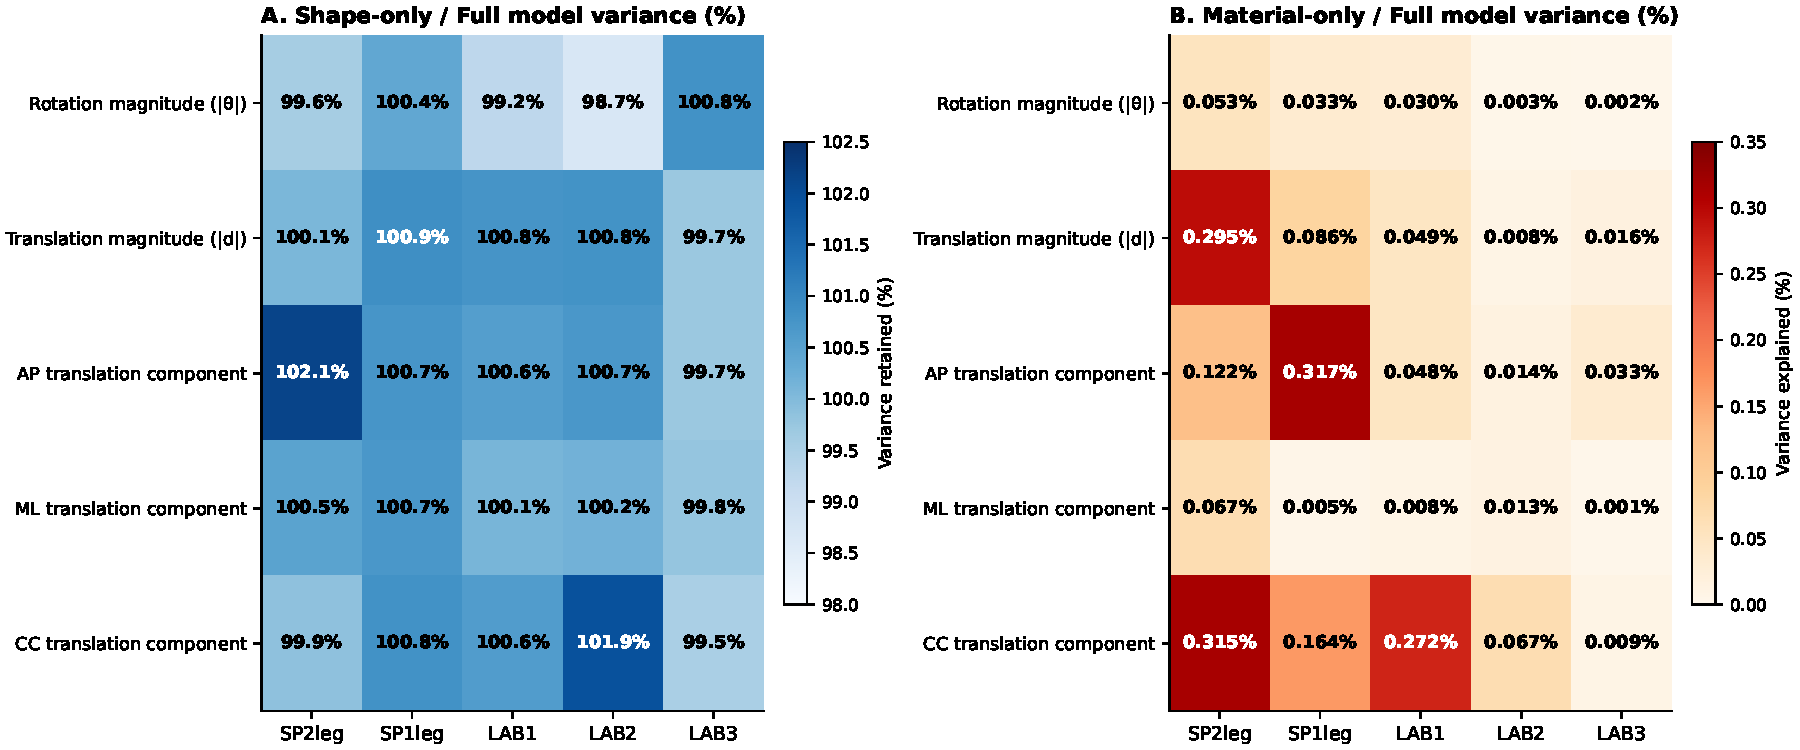
\includegraphics[width=0.98\textwidth]{figures/Fig5_variance_channels.pdf}
\caption{\textbf{Variance-channel decomposition: shape versus bone material heterogeneity.} Dual annotated percentage heatmaps displaying: (A) Proportion of full-model population variance retained by the shape-only model ($V_{\text{shape}} / V_{\text{full}} \times 100\%$). (B) Proportion of full-model variance explained by the material-only model ($V_{\text{material}} / V_{\text{full}} \times 100\%$). Cell annotations indicate exact percentages across five load cases and six kinematic metrics.}
\label{fig:variance}
\end{figure}

\subsection{Secondary allometric scaling with pelvic size}
Log--log power-law regressions of SIJ micromotion against total pelvic bone volume revealed load-dependent scaling (Table~\ref{tab:allometry}B; Fig.~\ref{fig:allometry}). Statistically significant negative allometric scaling was observed during single-leg stance (SP1leg): larger pelvic volume was associated with reduced micromotion in both sexes, with scaling exponents of $\beta_{\text{male}} = -0.482$ (95\% CI $-0.870$ to $-0.094$, raw $p = 0.0148$, FDR $q = 0.0742$) and $\beta_{\text{female}} = -0.428$ (95\% CI $-0.762$ to $-0.093$, raw $p = 0.0122$, FDR $q = 0.0405$) for rotation ($R^2 = 0.38$), and $\beta_{\text{male}} = -0.569$ (95\% CI $-0.869$ to $-0.269$, raw $p < 0.001$, FDR $q = 0.0020$) and $\beta_{\text{female}} = -0.432$ (95\% CI $-0.669$ to $-0.194$, raw $p < 0.001$, FDR $q = 0.0037$) for translation ($R^2 = 0.50$).

Under two-leg stance and parturition configurations, volume scaling exponents were generally attenuated, with 95\% confidence intervals crossing zero in most cases. A notable exception was female translation in LAB2, which retained a statistically significant negative scaling exponent ($\beta_{\text{female}} = -0.614$, 95\% CI $-1.061$ to $-0.166$, raw $p = 0.0072$, BH-FDR $q = 0.0360$), whereas male scaling in LAB2 was not significant ($\beta_{\text{male}} = -0.367$, 95\% CI $-0.904$ to $0.171$, $p = 0.1809$, $q = 0.3654$). Crucially, sex-by-size interaction terms were not statistically significant across any load case or outcome after BH-FDR correction (all corrected $q \ge 0.958$), indicating that male and female pelves follow consistent allometric scaling trajectories.

In pooled cluster-robust models across all 1,390 observations, translation magnitude exhibited an overall negative volume association ($\beta = -0.092$ per 1 SD increase, 95\% CI $-0.143$ to $-0.041$, BH-FDR $q < 0.001$; Table~\ref{tab:allometry}A), modulated by significant load$\times$size interaction terms.

\begin{figure}[H]
\centering
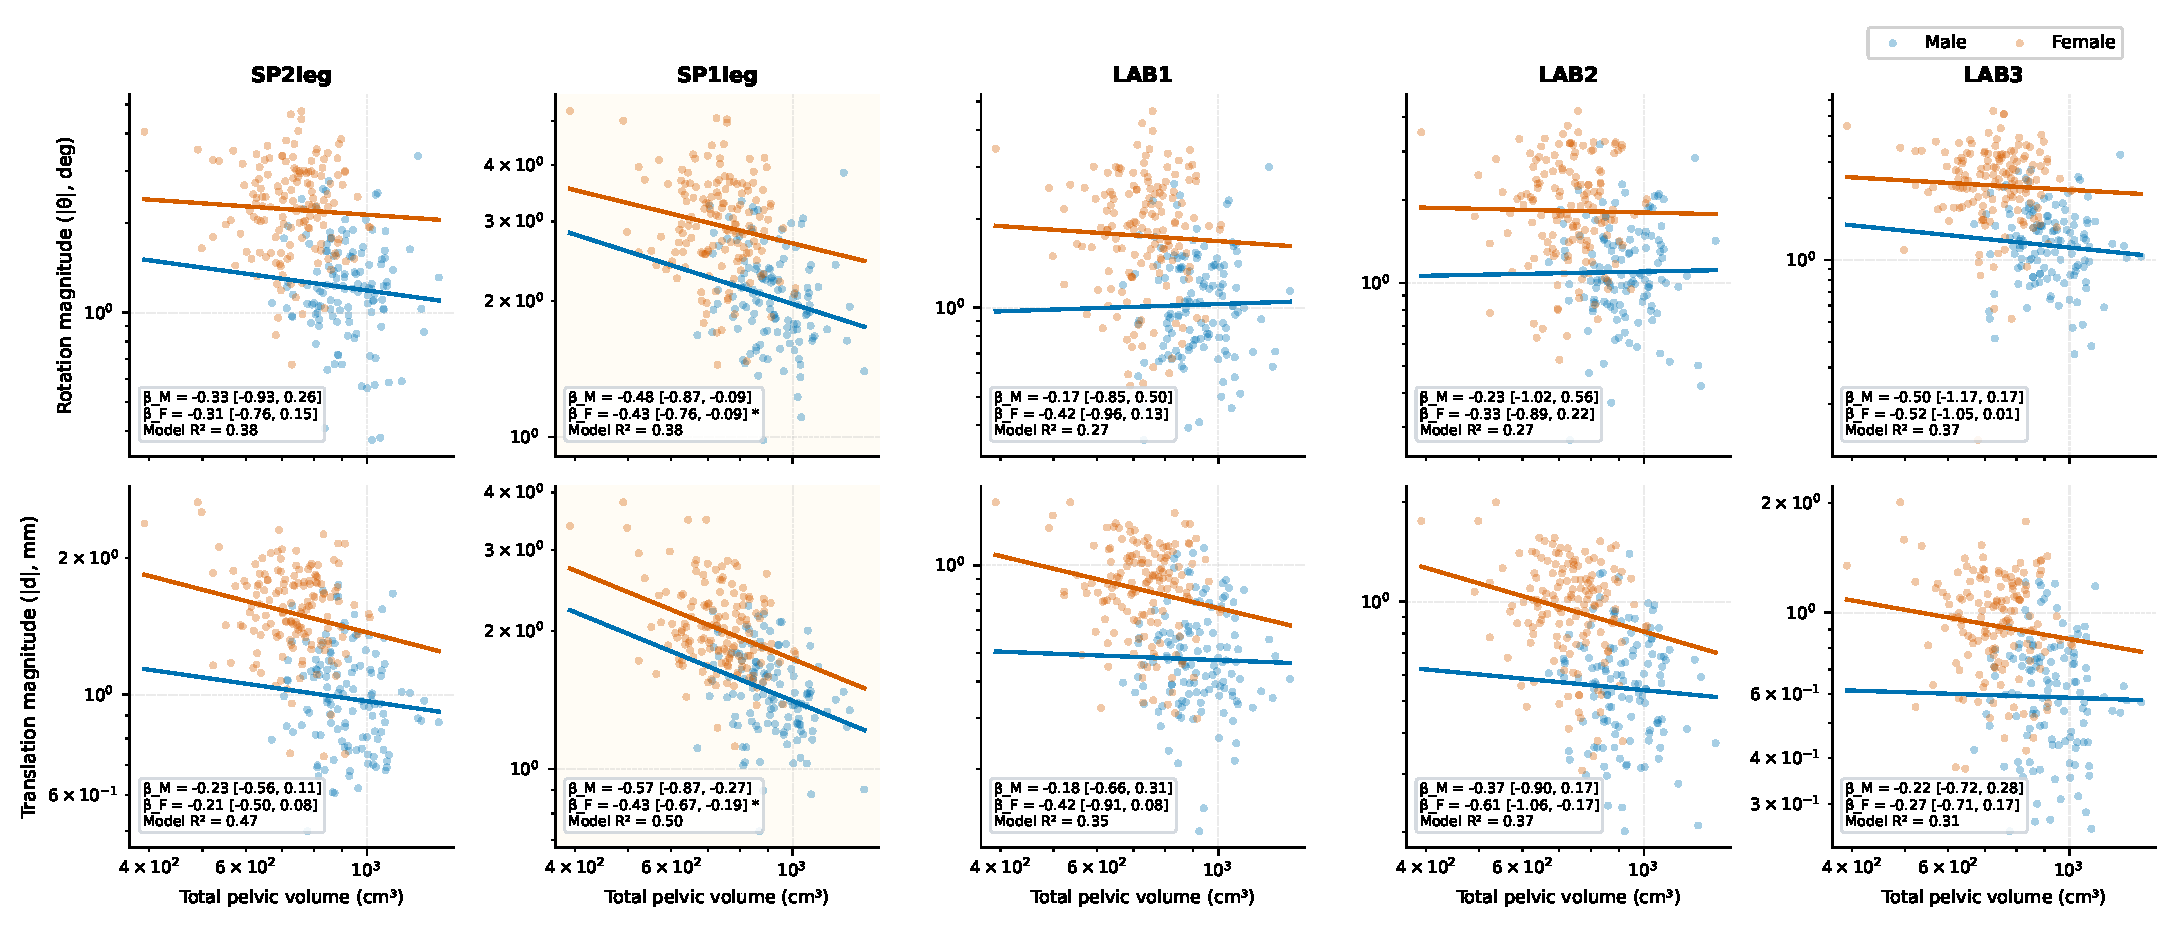
\includegraphics[width=0.98\textwidth]{figures/Fig6_allometry_loglog.pdf}
\caption{\textbf{Allometric log--log scaling of SIJ micromotion with total pelvic volume.} $2\times 5$ regression grid for rotation magnitude (top) and translation magnitude (bottom) across SP2leg, SP1leg, and LAB1--LAB3. Points show male (blue) and female (vermilion) subjects; solid lines depict sex-stratified power-law fits. The shaded panel highlights single-leg stance (SP1leg), which displays consistent negative allometric scaling in both sexes.}
\label{fig:allometry}
\end{figure}

\begin{table}[H]
\centering
\caption{Pooled cluster-robust regression models and load-wise allometric scaling exponents. Panel A: Pooled models across all 1,390 observations (clustered by subject). Panel B: Load-specific log--log power-law scaling exponents ($\beta$ and 95\% CI).}
\label{tab:allometry}
\textbf{Panel A}\par
\StdTableInput{tables/generated/table4a_primary_models.tex}
\vspace{1em}

\textbf{Panel B}\par
\StdTableInput{tables/generated/table4b_allometry.tex}
\end{table}

\subsection{Summary of hypothesis testing}
In summary:
\begin{itemize}
\item \textbf{H1 (Load-Dependence and Stance Asymmetry): Supported.} Locomotor loading engaged self-bracing nutation ($\theta_{\text{nut}} \ge 1.06^\circ$), with SP1leg driving a substantial increase in bilateral translation asymmetry ($2.01$~mm vs.\ $0.21$~mm) and frontal tilt. Parturition proxies reduced sagittal nutation ($0.41^\circ$--$0.43^\circ$) and re-routed displacement into transverse expansion.
\item \textbf{H2 (Directional Kinematic Contrasts): Supported.} Parturition loading reduced vertical craniocaudal shear ($\Delta\text{CC} \le -0.85$~mm) while selectively augmenting transverse distraction ($\Delta\text{ML} \ge +0.09$~mm) and sagittal gliding.
\item \textbf{H3 (Sex-Related Differences and Morphometric Associations): Supported.} Female pelves exhibited greater translational compliance across labor configurations ($+0.19$ to $+0.23$~mm in fully adjusted models, $p \le 0.020$). This difference attenuated upon adjusting for pelvic size and architecture, and correlated positively with subpubic arch angle ($r = 0.52, p < 10^{-19}$).
\item \textbf{H4 (Relative Contributions of Shape versus Material Heterogeneity): Supported.} Macroscopic skeletal geometry accounted for 98.7\% to 102.1\% (median 100.5\%) of population variance, whereas bone mineral density heterogeneity explained less than 0.32\% (median 0.033\%). Allometric volume scaling was load-dependent, manifesting most clearly during single-leg stance.
\end{itemize}
